\documentclass[bachelor,fontset=fandol,AutoFakeBold=true]{nuaathesis}

%%======================================
%% 此段代码用于将脚注放在页脚线下,考虑到有同学会认为当前的方式比较丑
%% 代码来源:
%% http://tex.stackexchange.com/questions/164367/how-to-make-footnotes-appear-at-bottom-of-the-footers-bar
% \makeatletter
% \renewcommand\footnoterule{%
%   \kern91.8\p@
%   \hrule\@width\linewidth
%   \kern2.6\p@}
% \makeatother
%% 使用此种方法不要超过四条脚注,第五条及以后的脚注无法显示
%% 使用此种方法第一行的脚注不要过长,否则会覆盖页脚的页码
%%======================================

\usepackage{systeme}

\addbibresource{bib/sample.bib}

\begin{document}
\title{利用线性代数和优化知识求解PnP和ICP问题}
\author{1823002班 \\ 丁楚原}
\date{\today}
\maketitle

\frontmatter                            %% 使用罗马数字对摘要页编号
\tableofcontents                   %% 目录、图目录、表目录
%% 中文摘要,{}中是中文关键词
\begin{abstract}{线性代数;机器视觉;相机位姿解算;PnP;ICP.}
在机器视觉和导航控制领域,相机位姿为求解是一项基本的工作,
只有在获得了相机位姿之后才能计算机器人的位置,并对其运动进行决策和规划。
在本文中,我们将从线性代数理论介绍两种求解相机位姿的方法:PnP和ICP方法,
其中前者是使用普通RGB相机进行计算的,后者是使用了深度相机(双目或ToF)计算的。
本文大量使用了线性代数和优化理论的知识\footnote{也是本人这学期上的三门数学课之二},
但是限于知识储备不足,过于复杂的证明请查看参考文献。
得益于开源社区,这些算法的实践并没有数学推导看起来那么困难。
\end{abstract}
\mainmatter                             %% 使用阿拉伯数字对正文编号
\pagestyle{plain}                   %% 正文内容

\chapter{机器视觉知识概述}
机器视觉是指使用计算机模拟人类视觉系统来对现实世界中的物体、场景进行感知和理解的技术。
它涉及图像采集、处理、分析以及基于这些图像的决策和行为。
具体来说,机器视觉系统通常包括以下几个组成部分:
图像采集:通过摄像头或其他成像设备获取图像。
图像处理:对采集到的图像进行预处理,如去噪、增强、二值化等,以提高后续分析的准确性。
图像分析:识别图像中的特征或对象,进行测量、分类、识别等操作。
决策和行为:根据图像分析的结果,做出相应的决策或执行特定的操作。
机器视觉的目标是使计算机能够“看”到物体并理解其意义,从而在没有人工干预的情况下完成各种任务。

\section{坐标系与物体位姿}

我们在机器视觉中使用三个坐标系:
\begin{enumerate}
    \item 图像坐标系
    \item 相机坐标系
    \item 世界坐标系
\end{enumerate}
除了图像坐标系是二维平面,其他两个坐标系都是三维空间。
对于三维坐标系下的某个物体,要准确描述其位姿需要六个参数,即六个自由度。
为了方便运算,我们一般将其化为四元数进行计算和设备之间的传输。


\section{相机模型}
相机将三维世界中的坐标点投影到二维平面上,并用一组参数来描述投影的位置、方向、视野等。我们这里使用到的是\textbf{针孔模型}。
\begin{figure}[htbp]
    \centering
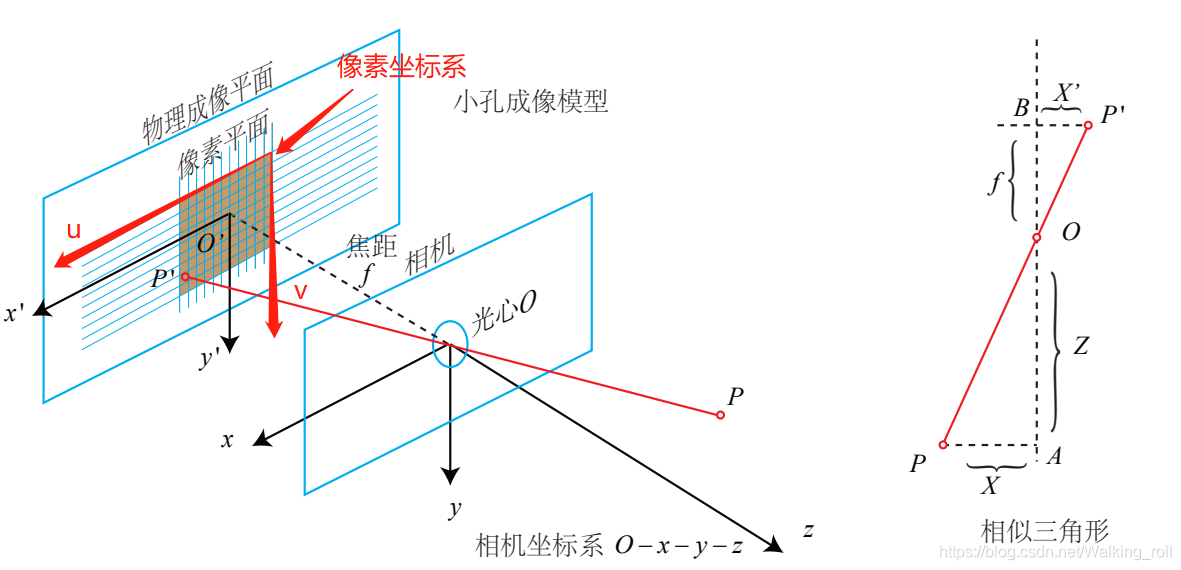
\includegraphics[width=0.5\textwidth]{figures/针孔相机.png}
\caption{针孔相机模型}
\end{figure}

这里我们定义两个坐标系:\textbf{图像坐标系}和\textbf{相机坐标系}。

具体定义方式为:图像坐标系的原点$O'$位于图像左上方,其$u$轴、$v$轴分别与$x'$,$y'$轴平行且方向相同。
像素坐标和成像平面之间,相差了缩放和平移的关系,这个关系可以用\textbf{线性变换}来表示。
我们设坐标在$u$轴上缩放了$\alpha$倍,在$v$轴上缩放了$\beta$倍,同时原点相对光轴平移了$[c_x,c_y]^T$。
则图像坐标系到相机坐标系的变换可以表示为:

\begin{equation}
\begin{cases}
    u = \alpha X' + c_x \\
    v = \beta Y' + c_y 
 \end{cases}
\end{equation}

根据初中学的小孔成像公式,带入镜头透镜x、y方向的焦距$f_x$、$f_y$,我们就可以得到:

\begin{equation}
    Z
    \begin{pmatrix}
        u \\ v \\ 1
    \end{pmatrix}
    =
    \begin{pmatrix}
        f_x & 0 & c_x \\
        0 & f_y & c_y \\
        0 & 0 & 1
    \end{pmatrix}
    \begin{pmatrix}
        X \\ Y \\ Z
    \end{pmatrix}
    \equiv K  P.
\end{equation}

我们把$K$称为\textbf{相机内参矩阵},内参是相机生产时刻确定的,与相机本身的特性无关。
同时$P$是相机在自身坐标系下的坐标,在真实情况下,我们通过世界坐标系来描述机器人的空间位姿,因此需要将$P$转换到相机坐标系。

其实,工程上使用的相机镜头是变化的,我们还需要进行标定获得更加准确的相机内参,但是本文假定已经完成了标定获得了准确的内参。

\begin{equation}
    Z P = Z 
    \begin{pmatrix}
        u\\v\\1
    \end{pmatrix}
    = K ( R P_{world} + t) = K T P_{world}
    \label{eq:rt}
\end{equation}

可以注意到,在相机的成像过程中我们将Z坐标归一化了,也就是失去了图像的深度信息,这对SLAM是十分致命的。
所以我们有两种路线解决这个问题:1、通过多个平面数据来源计算恢复深度信息;2、改进技术,使用能获得深度信息的相机。

\textbf{PnP就是一种选择第一个路线的算法}。


\chapter{PnP问题的建模与求解}
PnP(Perspective-n-Point)是求解3D到2D点对运动的方法。它描述了当知道n个3D空间点及其投影位置
时如何估计相机的位姿。我们在已知固定的路径点和及其视觉特征时,可以利用PnP求解相机的位姿。

PnP问题有很多种求解方法,这里介绍两种方法:直接线性变换(DLT)和使用非线性优化的光束平差法(Bundle Adjustment,BA)。

\section{直接线性变换法}

现在需要解决的问题是:我们知道一组3D点的位置,以及他们在某个相机中的投影位置,求解改相机的位姿。如果把3D点看作另一个相机坐标系中的点的话
则也可以求解两个相机相对运动。

我们从方程\ref{eq:rt}中可以得到:
\begin{equation}
    s \begin{pmatrix}
        u_1 \\ v_1 \\ 1
    \end{pmatrix}
    =
    \begin{pmatrix}
        t1 & t2 & t3 & t4 \\
        t5 & t6 & t7 & t8 \\
        t9 & t10 & t11 & t12 
    \end{pmatrix}
    \begin{pmatrix}
        X \\ Y \\ Z \\ 1
    \end{pmatrix} = T P
\end{equation}

其中T的矩阵是增广矩阵$[R|t]$,它包含了旋转矩阵和平移向量。用最后一行把s消去,得到:
\[
u1 = \frac{t1X + t2Y + t3Z + t4}{t9X + t10Y + t11Z + t12},\quad v1 = \frac{t5X + t6Y + t7Z + t8}{t9X + t10Y + t11Z + t12}
\]
为了简化表示,定义T的行向量为:
\[
t1 = [t1,t2,t3,t4]^T,\quad t2 = [t5,t6,t7,t8]^T,\quad t3 = [t9,t10,t11,t12]^T
\]
于是有:
\[
t1^T P  - t3^T P u1 =0,\quad t2^T P - t3^T P v1 =0
\]

如果有n个特征点对,那么我们有2n个方程,需要求解的参数有12个,所以能求解出$[R|t]$的最少点对是6对。

\textbf{当超过6对时,我们就可以使用课上学过但是不考的十分有用的SVD分解来求解这个超定方程。}

\section{最小化重投影误差求解PnP}

考虑n个三维空间点P及其投影p,我们希望计算相机的位姿R和t,可以用矩阵T表示。假设某个空间点的坐标为$P_i = [x_i,y_i,z_i]^T$
,其在相机坐标系中的投影为$p_i = [u_i,v_i]^T$。其关系如下:
\begin{equation}
    s_i \begin{pmatrix} u_i \\ v_i \\ 1 \end{pmatrix} = K T \begin{pmatrix}
    X_i \\ Y_i \\ Z_i \\ 1
    \end{pmatrix}
\end{equation}
也就是: 
$s_i u_i = K T P_i$

但是,由于相机位姿位置以及观测点的噪声,该等式存在一个误差,我们把误差求和,构建最小二乘问题
,并对其最小化:
\begin{equation}
    T^* = \arg min  \frac{1}{2} \sum_{i=1}^{n} \left( u_i - K T P_i \right)^2
\end{equation}

当然,这个问题的求解不是我现在具备的数理基础
\footnote{需要的用到的知识:抽象代数(群论部分),矩阵论,优化理论(列文伯格——马夸尔特方法等)}
能解决。

值得庆幸的是,参考书\footnote{《视觉SLAM十四讲》,高翔等著,视觉导航必读之作}给出了解答。



\chapter{ICP问题}
PnP问题是知道3D-2D对应点求解相机位姿,而ICP问题则是知道3D-3D对应点求解相机位姿。

在使用雷达或者深度相机时,我们可以获得视角的深度信息,这样如果知道固定的3D点,
那么我们就能得到3D-3D对应点。

\section{SVD方法}
假设我们有一组匹配好的3D点:
\begin{center}
$P = {p_1, p_2,..., p_n} , \quad P' = {p'_1, p'_2,..., p'_n}$
\end{center}
我们要找到一个欧氏变换$R,t$,使得
\begin{center}
$\forall i, \quad p_i = R p'_i + t$
\end{center}
之后就可以定义第i点的误差项:

\begin{equation}
    e_i = p_i - (R p'_i + t)
\end{equation}
建立最小二乘问题,使得误差的平方和达到极小的$R,t$:
\begin{equation}
\min \limits_{R,t} \frac{1}{2} \sum_{i=1}^n ||p_i - (R p'_i + t)||_2^2
\end{equation}

下面来推导它的求解方法。首先,定义两组点的质心:
\begin{equation}
    p = \frac{1}{n} \sum_{i=1}^n p_i, \quad p' = \frac{1}{n} \sum_{i=1}^n p'_i.
\end{equation}
之后,展开并化简误差项:
\[
\begin{split}
    & \frac{1}{2} \sum_{i=1}^{n} || p_i - (R p'_i + t) ||^2 \\
    &= \frac{1}{2} \sum_{i=1}^{n} || p_i - R p'_i - t + p - R p' + p - R p' ||^2 \\
    &= \frac{1}{2} \sum_{i=1}^{n} || (p_i - p - R(p'_i - p')) + (p - R p' - t) ||^2 \\
    &= \frac{1}{2} \sum_{i=1}^{n} || p_i - p - R(p'_i - p') ||^2 + || p - R p' - t ||^2 +  2 (p - R p')^T (p_i - p - R(p'_i - p'))
\end{split}
\]
注意到交叉线项部分$(p_i - p - R(p'_i - p') )$求和为零,我们可以把优化目标函数化简为:
\begin{equation}
    \min \limits_{R,t} \frac{1}{2} \sum_{i=1}^n || p_i - p - R(p'_i - p') ||^2 + || p - R p' - t ||^2
\end{equation}
发现左边之和旋转矩阵R有关,而右边同时含有R和t,但之和质心有关。我们只要获得了R,令第二项为零就能得到t。
于是优化的过程为:
\begin{center}
    \begin{tabular}{l l}
        \hline
        步骤 & 操作 \\
        \hline
        1.计算每个点去质心坐标 & $q_i = p_i - p , q'_i = p'_i - p'$ \\
        2.建立以下优化问题计算R & $R^* = arg \min \limits_{R} \frac{1}{2} \sum_{i=1}^n ||q_i - Rq'_i||^2$ \\
        3.从R计算t & $t = p - R p'$ \\
        \hline
    \end{tabular}
\end{center}
这个过程中的优化问题R的误差项展开可得
\begin{equation}
    \frac{1}{2} \sum_{i=1}^n (q_i^T q_i + q^{'T}_i R^T R q_i - 2 q_i^T R q'_i)
\end{equation}
因为第一项和R无关,第二项$R^T R = I$,亦与R无关,所以优化问题可以简化为:
\begin{equation}
    \sum_{i=1}^n -q_i^T R q'_i = \sum_{i=1}^n - tr(R q'_i q_i^T) = - tr(R \sum_{i=1}^n q'_i q_i^T)
\end{equation}

计算这个最优问题即可解出答案。

\chapter{总结、实践与致谢}
本文推导了PnP和ICP问题的模型建立与求解过程,其中PnP求解给出了两种方法,
实际上,根据特征点对的性质不同,还有很多求解方法,如:P3P,EPnP,UPnP等;
ICP问题也可以使用非线性优化的方法求解。

在实际工程中,我们可以使用开源库OpenCV中的solvePnP和solvePnPRansac函数求解PnP问题,
针对优化问题求解,在g2o、ceres、eigen等库的帮助下,我们可以快速地实现求解。

这里提供一个作者比赛\footnote{我们队伍地githup地址为:\url{https://github.com/nuaa-rm}}中的实践,这是通过RGB信息一个识别方形框六自由度的问题,
在尺度归一化的约束下,可以准确的算出目标的欧拉角。项目地址为:\url{https://github.com/happyADD/ENG2025.git}
这个项目基于ROS2建立,使用了海康威视的相机。

本学期是我学习的线性代数可谓是十分重要的一门课,曾经在一本专业书中看到过这样一句话:
\textbf{“工程师的一生要学三次线性代数:一次是为了考试,一次是为了研究,一次是为了实践。”}
\footnote{没记错应该是看书看到的,或许大约不是我梦里想出来的。}
这个学期我在学习《解析几何与线性代数A》的同时也学了《最优化方法》、《微分方程A》两门数学课,
同时还在完成着上面提到的比赛项目。如果这门课算是第一次,两外两门课算是第二次,自己的小项目算是第三次的话,
可以说,我用一个学期的实践完成了三次线性代数的学习!
\footnote{虽然以后肯定还要更加深入的学,但是四舍五入多活了三四十年。}
也感谢这学期的三位数学老师,是你们的有条理的一步一步推导让我知道更多。


\backmatter                             %% 文后无编号部分
\printbibliography[heading=bibintoc]
\end{document}
